%%%%%%%%%%%%%%%%%%%%%%%%%%%%%%%%%%%%%%%%%%%%%%%%%%%%%%%%%%%%%%%%%%%%%%%%
\chapter{Design} \label{Design}
%%%%%%%%%%%%%%%%%%%%%%%%%%%%%%%%%%%%%%%%%%%%%%%%%%%%%%%%%%%%%%%%%%%%%%%%
Our system leverages a novel approach for efficient dynamic cache updates for improved inference latency and throughput.
We design a single-machine, multi-GPU inference system and build upon caching techniques in GNN training systems discussed in the previous chapter. 
By focusing on single-machine inference, we can avoid network overheads and achieve better latency and throughput than distributed systems when graph size is appropriate.

In this chapter, we address three key research questions:
\\ \\
\noindent \textbf{RQ1: How can GPU feature caches effectively capture GNN inference patterns?} \\
Section \ref{Design: Towards Dynamic Caching} describes opportunities for dynamic caches to outperform existing static caches at inference time and highlights the shortcomings of naive approaches. Section \ref{Design: Policy} proposes a frequency-based cache admission and eviction policy that produces better cache hit rates than static baselines while offering a path toward efficient update operations.
\\ \\
\noindent \textbf{RQ2: How can the impact of dynamic cache updates on request-response latency be minimized?} \\
Section \ref{Design: Async Update} details how we derive an asynchronous cache update mechanism based on profiling of a naive cache update mechanism using "prefetching". By carefully engineering this asynchronous cache update, we are able to hide cache update operations that would otherwise negatively impact tail latency.
\\ \\
\noindent \textbf{RQ3: How can we effectively leverage concurrency (multithreading, multi-GPU) to produce scalable inference?} \\
Since asynchronous updates synchronized using naive locking can produce blocking behaviors when pipelined (and thus no longer be truly asynchronous), we propose a lock-free mechanism to perform cache updates, discussed in Section \ref{Design: Lock-free}.
Lastly, Section \ref{Design: Multi-GPU} describes how we extend our system to support multiple GPUs connected by NVLinks and share a single logical cache.

% Our system implements the same frequency-based admission and eviction policy from the prefetching baseline but combines it with an asynchronous cache update mechanism to reduce tail latencies. 
% Section \ref{Design: Policy} analyzes this policy in more detail and Section \ref{Design: Async Update} describes how asynchronous updates take place. 
% Since asynchronous updates synchronized using naive locking can produce blocking behaviors when pipelined (and thus no longer be truly asynchronous), we propose a lock-free mechanism to perform cache updates, discussed in Section \ref{Design: Lock-free}.
% Lastly, Section \ref{Design: Multi-GPU} describes how we extend our system to support multiple GPUs connected by NVLinks and share a single logical cache.


%%%%%%%%%%%%%%%%%%%%%%%%%%%%%%%%%%%%%%%%%%%%%%%%%%%%%%%%%%%%%%%%%%%%%%%%
\section{Towards Dynamic Caching} \label{Design: Towards Dynamic Caching}
%%%%%%%%%%%%%%%%%%%%%%%%%%%%%%%%%%%%%%%%%%%%%%%%%%%%%%%%%%%%%%%%%%%%%%%%
One of our key observations is that effective caching is pivotal to reducing data loading costs, and dynamic cache policies can enable better cache hit rates.
We define a \textit{dynamic} cache policy as one that swaps node features in and out of GPU memory over time. We identify two key opportunities  that dynamic caches can capture that static caches neglect:
\begin{description}
    \item[Inference request locality] Inference requests generate large neighborhoods during the $k$-hop neighborhood generation process. Due to this, if inference requests being "close" in the graph have reasonable semantic meaning in the real world, then we can expect inference requests to exhibit locality. For example, in a social network graph there may be clusters of users who are in a similar geographic area. These users may have more activity and generate more inference requests during the daytime, meaning that subgraphs become "hot" at different points in time. Prior work in the graph processing space has also noted the importance of request locality in domains such as traffic prediction or knowledge graph mining \cite{QGraph_2018}.
    % For example [traffic], [over time], [popular products]
    \item[Sampling patterns] A degree-based policy only attempts to approximate the likelihood of encountering a node during inference. For example, a low-degree node that is directly adjacent to several high-degree nodes is likely to be similarly "hot" to its high-degree neighbors, due to GNNs requiring multi-hop neighborhoods. Additionally, certain GNN architectures may sample node neighbors using some other heuristics, such as sampling based on edge weight \cite{GAT_2018}.
\end{description}

\subsection{Why Traditional Dynamic Caches are Ineffective} \label{Design: strawman}
An intuitive first step towards dynamic caches is to consider using traditional cache eviction policies such as LRU, LFU, or FIFO. However, many of these approaches have too much overhead to be effective for GNN inference. 

In the GNN inference case, each request (comprising anywhere from one to several hundred target nodes) can generate $k$-hop neighborhoods of hundreds of thousands of nodes.
As a result, the overhead of cache replacement heuristics can quickly overtake any performance gains from improved cache hit rates. For example, the traditional implementation of an LRU cache using a linked list and hash table to track elements will severely bottleneck GNN inference. Consider the following back-of-the-envelope calculation. We find that a naive GNN inference system can generally serve requests with $< 100$ ms latency. Assuming a cache put or get takes only $500$ ns, as is the case with many publicly available LRU cache implementations \cite{HashiCorp_GoLang_LRU}, for one request this requires $~100,000 \text{ nodes} * ~500 \text{ ns} = 50 \text{ ms}$. Given that this would add at least $50\%$ to our original inference latency, such overhead is clearly unacceptable. 

To handle potentially huge neighborhood sizes, a key requirement for a cache policy is to be easily parallelizable. A frequency-based heuristic meets this criterion and has been shown to be effective in the GNN setting a training time, with GNNLab's pre-sampling approach \cite{GNNLab_2022}. Even so, the traditional LFU policy can still struggle versus a static cache baseline as it requires some kind of sorting or top-$k$ operation for each request served.

Furthermore, large neighborhood sizes require us to also consider a cache admission policy. If only a cache eviction policy is used, it is easy for a "one-hit wonder" to be brought in among hundreds of thousands of other nodes and waste cache space.

Note that static caches do not suffer from these performance problems since checking for cache hits is easily implemented using tensor operations.
% However, since LFU is only an eviction policy 
% only eviction policies, in practice can be subject to one-hit wonders
% Prefetch based approach

% We draw a distinction between cache policy and cache mechanism.

%%%%%%%%%%%%%%%%%%%%%%%%%%%%%%%%%%%%%%%%%%%%%%%%%%%%%%%%%%%%%%%%%%%%%%%%
\section{Frequency-based Admission \& Eviction Policy} \label{Design: Policy}
%%%%%%%%%%%%%%%%%%%%%%%%%%%%%%%%%%%%%%%%%%%%%%%%%%%%%%%%%%%%%%%%%%%%%%%%
Motivated by our observations in the previous section, in this section we propose a simple frequency-based cache admission and eviction policy. Then, we briefly illustrate the improved cache hit rates of this policy when using a naive, strawman cache update mechanism.

The goal of our policy is straightforward: to admit the most frequently occurring node features and evict the least frequent node features within a particular time window. Implementing this heuristic requires tracking node frequencies and decaying them over time.

In our implementation node frequencies are tracked in a buffer in GPU memory. By tracking frequencies on the GPU rather than the host, our system avoids an additional device to host copy, since computation graphs are built on GPU. The frequency buffer has length equal to the number of nodes in the graph.
Each index in the buffer corresponds to a node, and the value is a counter that gets incremented whenever the node's feature is required.
To reduce GPU memory usage, this buffer uses only one byte for each node. 
However, the size of the buffer still scales with the number of nodes in the graph. We note that frequencies can also be tracked using a probabilistic data structure like a counting bloom filter \cite{Bloom_Filter_2000} or count-min sketch \cite{CountMinSketch_2005}, but we do not implement this.
Using such a probabilistic data structure actually makes it easier to add new nodes into the graph, since there is no buffer that needs to be resized.
We leave this as future work.

To capture changes in node frequencies, the count buffer must decay over time.
This is implemented by periodically dividing all counts in the buffer by two, a technique adapted from TinyLFU \cite{TinyLFU_2014} which produces exponential decay.
A nice property of exponential decay is that it is easy to bound the maximum possible count and fit it within the one byte constraint. 
Additionally, the decay can be implemented as a bit shift for better performance and still works with a count-min sketch or counting bloom filter.

% There are many policy choices regarding how exactly to choose which nodes to evict or admit. 
% For example, a policy could weight both a node's degree as well as its recent frequency when making admission decisions. 
% The weighting of node degree versus frequency is a user-adjustable knob in our system, but for the evaluation in Chapter \ref{Evaluation}, we use only frequency when evaluating frequency-based approaches.


\subsection{Strawman Prefetching Mechanism}
Given the above policy, an actual implementation must choose some mechanism by which to perform cache updates and perform the top-$k$ frequency calculations. For example, LFU is traditionally implemented by tracking the most common elements using a heap and evicting/admitting into the cache per-request; however, as we saw earlier this can harm inference latency. We present an alternative strawman mechanism that essentially replaces the static cache with a new one every $k$ requests according to the above policy. We call this alternative baseline mechanism our \textit{prefetching} strawman. 

In particular, every $k$ requests the cache is entirely replaced with the most common nodes that appeared in the previous $k$ requests. This means that node features are pulled to the GPU feature cache and request handling must be paused as necessary. 

The key idea is that this strawman maintains the low overhead nature of a static cache while improving cache hit rates, but every $k$ requests it incurs a large penalty due to a cache update. This cache update penalty produces significant tail latency, which we analyze in the next section.

%%%%%%%%%%%%%%%%%%%%%%%%%%%%%%%%%%%%%%%%%%%%%%%%%%%%%%%%%%%%%%%%%%%%%%%%
\section{Asynchronous Cache Update mechanism} \label{Design: Async Update}
%%%%%%%%%%%%%%%%%%%%%%%%%%%%%%%%%%%%%%%%%%%%%%%%%%%%%%%%%%%%%%%%%%%%%%%%
 
To eliminate tail latencies associated with the prefetching strawman, our system uses an asynchronous cache update mechanism, moving cache update operations off the critical path when responding to inference requests.
Table \ref{Update latencies} provides a breakdown of average cache update overheads for a selected dataset, ogbn-products, during a single-threaded inference execution. The prefetching-based update produces significant tail latency, in this case increasing response latency by more than a third when the update occurs.

\begin{table}[h!]
    \begin{center}
        \textbf{Breakdown of Average Cache Update Overhead}
        \begin{tabular}{|c c c|} 
        \hline
        \textbf{Operation} & \textbf{Time (ms)} & \textbf{Percent of Update Time} \\ [0.5ex] 
        \hline\hline
        Update cache metadata & 2.7 & 47\%  \\
        \hline
        Feature copy & 2.2 & 38\% \\
        \hline
        Compute most common features & 0.6 & 10\% \\
        \hline
        Misc. (locking, device sync, etc.) & 0.2 & 3.5\% \\
        \hline
        Total & 5.7 & \\
        \hline
        \end{tabular} \\
        Average inference latency without update: 12.7 ms
    \end{center}
    
    % ogbn-products, uniform sampling, batch size 256, total latency 
    \caption{Breakdown of time spent on operations when performing cache update.
    These are the operations that contribute to significant tail latency with the prefetching policy.
    }
    \label{Update latencies}
\end{table}

The largest contributors to cache update overhead in the prefetching strawman are copying new features from host memory to GPU memory and updating cache metadata.
Using this profiling information, we motivate three design decisions.
\textbf{(1)} Rather than prefetching features to move into GPU memory, we move features into the cache only when they are needed by inference requests, similar to traditional cache eviction policies. 
\textbf{(2)} To sidestep overheads due to updating cache metadata, we move metadata updates to a separate host thread and CUDA stream (synchronization is discussed in Section \ref{Design: Lock-free}).
\textbf{(3)} Lastly, we can compute the most common features (in practice a top-$k$ operation) in a separate CUDA stream.

% \begin{enumerate}
%     \item Compute set of cache candidates
%     \item Python process places torch tensor into queue, picked up by C++ thread
%     \item Removed from queue when model execution finishes to avoid ballooning memory usage
%     \item Also experimented with updating counts/doing other operations in C++ thread
% \end{enumerate}

\subsection{Computing Cache Candidates} \label{Design: Cache candidates}
To support moving features into the cache only when they are needed by inference requests while adhering to the desired policy, we introduce the idea of \textit{cache candidates}, a set of node ids computed every $k$ requests. When a cache miss occurs and new node features are copied to the GPU from host memory, the new features are checked against the set of cache candidates. If a feature corresponds to a node that is a cache candidate, then it will replace a non-cache candidate present in the cache. This is possible since at any given point in time, the number of cache candidates is equal to the size of the cache.


\subsection{Performing Cache Updates}
Cache metadata updates actually comprise the majority of the tail latency we are trying to avoid. 
The main metadata update is simply correctly computing which indices of the cache correspond to new features and correctly updating another tensor that maps node ids to their index in the cache.

We perform these metadata-related operations, along with the cache replacement described in the previous section, in a separate host thread than the one handling inference requests. 

One important aspect of this approach is that the cache update should occur during the model forward pass.
The key insight is that node features are already present in GPU memory for the model forward pass and thus are assumed to fit in GPU memory fine.
However, if the asynchronous update thread holds on to these tensors longer than the model forward pass would normally take, memory usage can be inflated. 
We avoid this problem by allowing the model forward pass to have full ownership of any node features required for computation.
If the model forward pass for a given inference request is completed and the cache update has not started, then the cache update will be ignored.

To further avoid contention of GPU compute due to cache updates happening concurrently with model computation, we assign the cache update operations to a lower priority CUDA stream than model computation.

%%%%%%%%%%%%%%%%%%%%%%%%%%%%%%%%%%%%%%%%%%%%%%%%%%%%%%%%%%%%%%%%%%%%%%%%
\section{Lock-free Cache Updates} \label{Design: Lock-free}
%%%%%%%%%%%%%%%%%%%%%%%%%%%%%%%%%%%%%%%%%%%%%%%%%%%%%%%%%%%%%%%%%%%%%%%%
Asynchronous cache updates naturally raise concerns about correctness and performance due to concurrency. While naive locking may initially be adequate, at scale this may not be the case. In this section we look at a novel lock-free approach using \textit{masking} to avoid lock contention due to cache updates.


Consider the case where we would like our system to be pipelined to maximize throughput. Since the data loading stage requires reading from the cache, we must be careful about synchronization between cache updates and data loading since cache updates are not atomic.
\begin{figure}[h!]
    \centering
    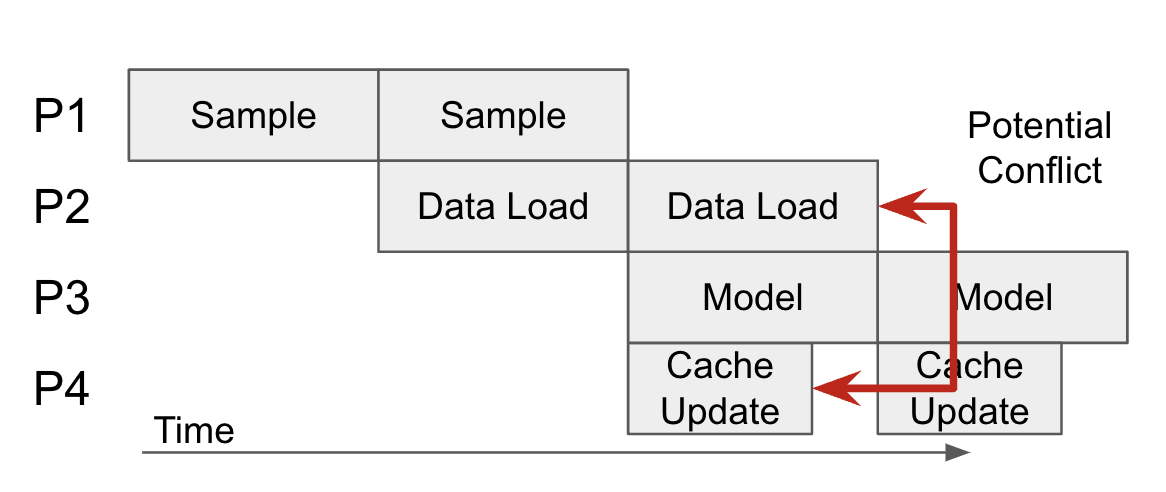
\includegraphics[width=0.85\textwidth]{figures/Pipeline no lock.png}
    \caption{Ideal pipelining with potential race condition}
    \label{Impl: Conflict pipeline}
\end{figure}     
A case such as the one illustrated in Figure \ref{Impl: Conflict pipeline} can lead to cache readers reading the wrong feature from the cache if a cache update changes the cache buffer before the reader completes. 

A naive approach is to use mutual exclusion, such as with a reader-writer lock, but this can lead to asynchronous updates having equivalent performance to the original synchronous variety. Figure \ref{Impl: Contended pipeline} illustrates this effect. In this example, by enforcing mutual exclusion between the data loading thread and cache update thread, the second inference request is forced to wait on the cache update from the first inference request, meaning the latency of the first cache update was simply "passed along".

\begin{figure}[h!]
    \centering
    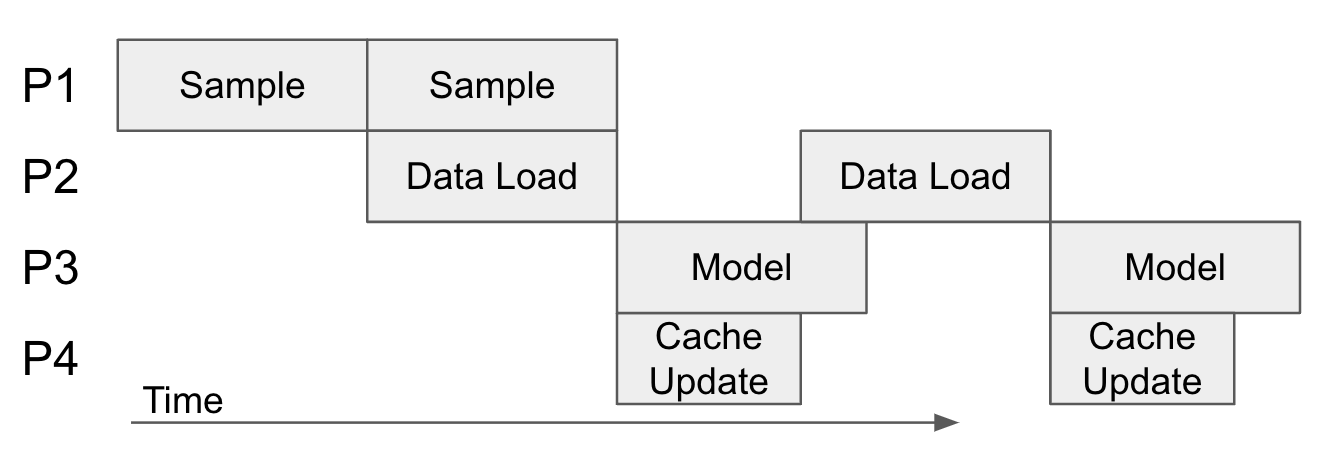
\includegraphics[width=\textwidth]{figures/Pipeline with lock.png}
    \caption{Pipeline stall due to enforcement of mutual exclusion between cache update and data loading stages}
    \label{Impl: Contended pipeline}
\end{figure}    

Even with a read-preferring or write-preferring reader-writer lock, eventually it must be the case that a cache read waits for a cache update, causing this "latency passing" behavior.  

\subsection{Masked Updates}
Motivated by the key observation that readers should be wait-free but writers can wait, we introduce a novel alternative to mutual exclusion in this context. In our approach, which we call \textit{masking} cache updates, update threads preemptively \textit{mask away} cache entries from cache readers and only perform updates once these cache entries will no longer be used by readers. 

Note that we assume only one thread performs a cache update at a time (per GPU), which is enforced by a simple mutex per GPU. If a cache update thread fails to acquire the lock, the update is thrown away.

To perform masked updates, we first add a \textit{mask} tensor to our cache metadata, which indicates for each node in the graph whether it is present in the cache (1 for present, 0 for not).

Then, for each logical thread of execution in the system, we initialize a start and finish atomic integer that just tracks whether the thread is currently performing a cache read.
When reading from the cache, threads will first increment their respective start atomic and then check the cache mask and only look in the cache for node ids where the mask indicates it is present.
Once the cache read is finished, the finish atomic is incremented.
Algorithm \ref{Design: Alg: Cache Read} summarizes this procedure.

When a cache update needs to occur, the writer will first blind write zeros into the cache mask for any node ids that will be evicted from the cache. 
Once the blind write has completed, the writer will then capture the value of all start atomics.
The writer capturing these values serves as a linearization point, as the writer will wait on the finish atomics until any in-progress reads complete. 
At this point the cache writer is certain that any cache indices that will be replaced are no longer in use by any cache readers.
Algorithm \ref{Design: Alg: Cache Write} summarizes this procedure.


% declaration of the new block
\algblock{ParFor}{EndParFor}
% customising the new block
\algnewcommand\algorithmicparfor{\textbf{parallel for}}
\algnewcommand\algorithmicpardo{\textbf{do}}
\algnewcommand\algorithmicendparfor{\textbf{end\ parallel for}}
\algrenewtext{ParFor}[1]{\algorithmicparfor\ #1\ \algorithmicpardo}
\algrenewtext{EndParFor}{\algorithmicendparfor}

\begin{minipage}{0.4\textwidth}
    \begin{algorithm}[H]
        \centering
        \caption{Cache Read} \label{Design: Alg: Cache Read}
        \footnotesize
        \begin{algorithmic}[1]
        \Procedure{Read}{$node\_ids$}
            \State $i \gets \text{ Reader thread id}$
            \State $S[i] \gets S[i] + 1$
            \ParFor{$node\_id \in ids$}
                \If{$mask[node\_id] = 1$}
                    \State Do cache read for $node\_id$
                \EndIf
            \EndParFor
            \State $F[i] \gets F[i] + 1$
        \EndProcedure
        
        \end{algorithmic}
    \end{algorithm}
\end{minipage}
\hfill
\begin{minipage}{0.5\textwidth}
        \begin{algorithm}[H]
            \centering
            \caption{Cache Write} \label{Design: Alg: Cache Write}
            \footnotesize
            \begin{algorithmic}[1]
            \Procedure{Update}{$admit\_nids, evict\_nids$}
                \State $mask[evict\_nids] = 0$
                \For{$reader\_id \in reader\_ids$}
                    \State $s'[reader\_id] \gets s[reader\_id]$
                \EndFor
                \While{$\exists id \in reader\_ids : s'[id] < f[id]$}
                    \State Wait
                \EndWhile
                \State Do cache update
                \State $mask[admit\_nids] = 1$
            \EndProcedure
            
            \end{algorithmic}
        \end{algorithm}
\end{minipage}

\begin{figure}[h!]
    \centering
    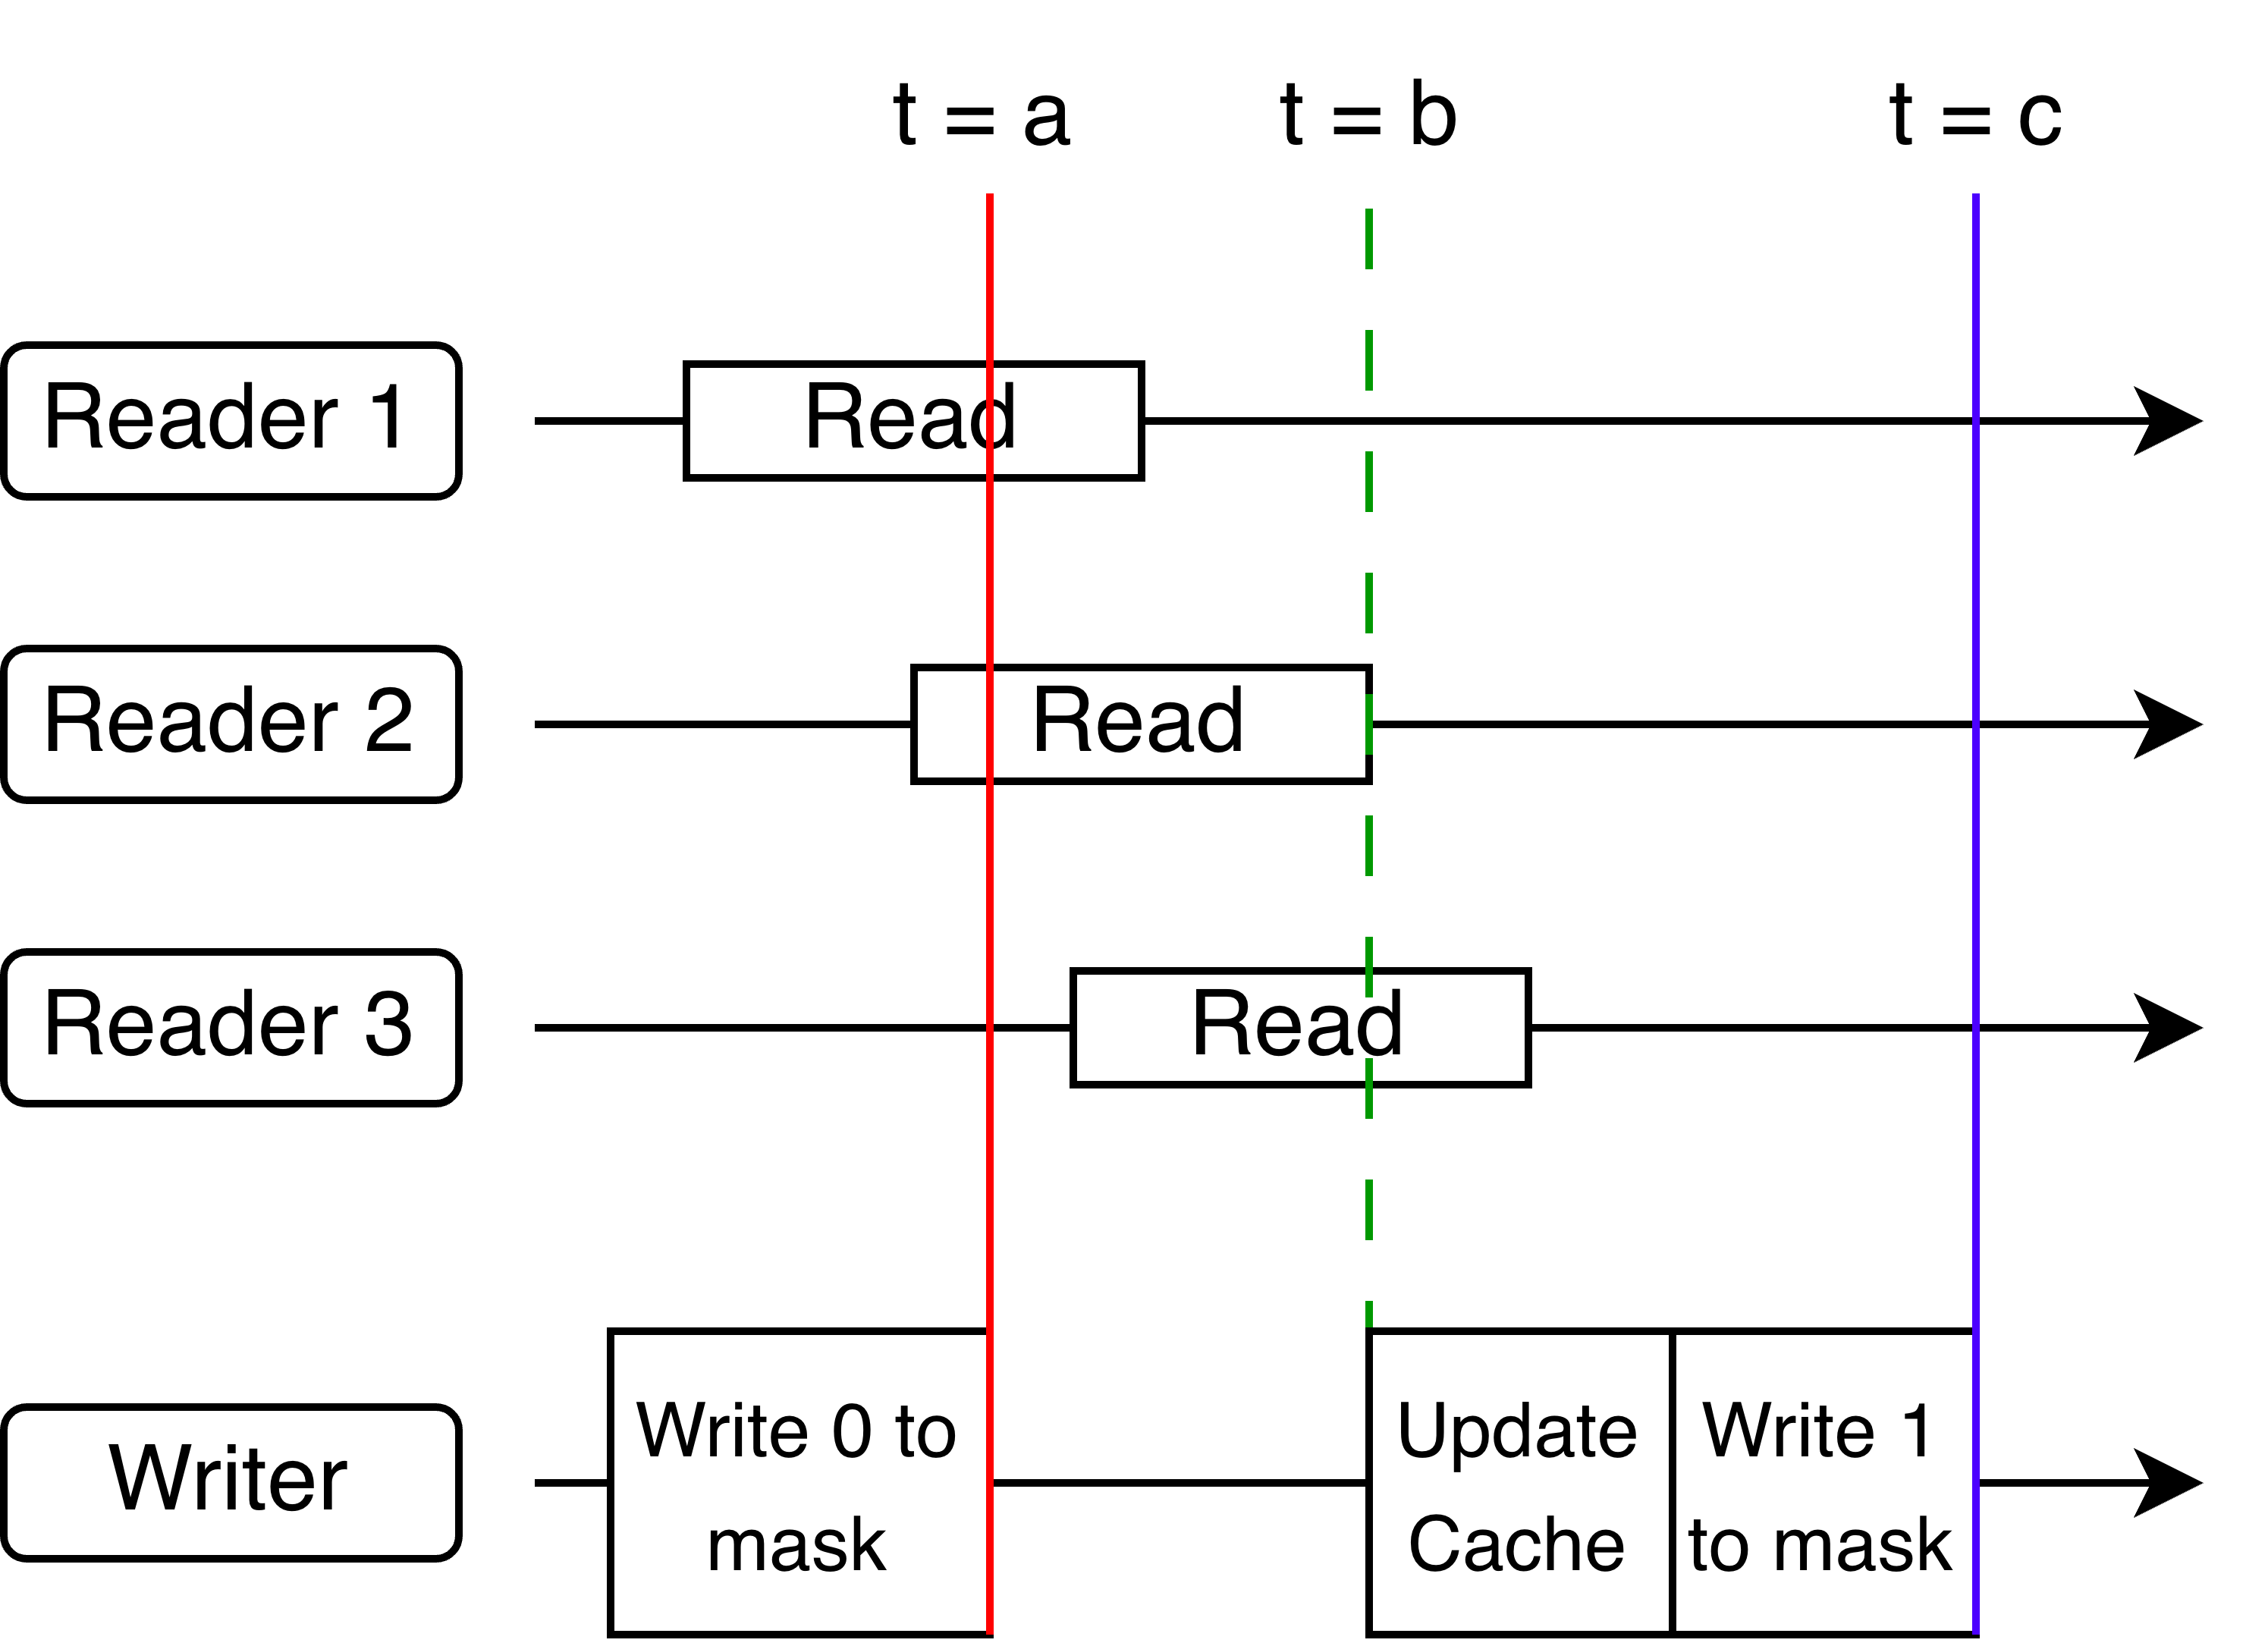
\includegraphics[width=0.7\textwidth]{diagrams/group_meeting_gnn-Multi-GPU.png}
    
    \caption{Readers and writers with masked, lock-free cache update}
    \label{Design: Lock-free update diagram}
\end{figure}    
Figure \ref{Design: Lock-free update diagram} provides a concrete example of this mechanism in a system with four threads of execution. At time $a$, the writer thread will capture the start atomics of each of the readers and wait for Reader 1 and Reader 2 to finish. At time $b$, the writer thread can start the cache update. Note that there is no actual conflict between Reader 3 and the writer thread since Reader 3 will have observed the initial cache mask update of the writer. However, Reader 3 may be subject to some false negatives as a result. Once the write procedure completes at time $c$ completes, the newly updated cache features are now globally visible.

%%%%%%%%%%%%%%%%%%%%%%%%%%%%%%%%%%%%%%%%%%%%%%%%%%%%%%%%%%%%%%%%%%%%%%%%
\section{Multi-GPU Cache Sharing} \label{Design: Multi-GPU}
%%%%%%%%%%%%%%%%%%%%%%%%%%%%%%%%%%%%%%%%%%%%%%%%%%%%%%%%%%%%%%%%%%%%%%%%
To maximize usage of available GPU memory, we support sharing of a single logical cache shared among multiple GPUs when connected by NVLink.
We use a simple hash partitioning scheme to partition node ids among multiple GPU caches. This means a node's feature can only ever be present in a single GPU's cache.

BGL implements a similar shared cache solution, but serializes all reads and writes to a particular GPU in a single thread to avoid synchronization problems. However, with the lock-free cache update solution described in the previous section, we allow for unlimited concurrent readers for any GPU's cache at a given time. The only restriction is that there can only be a single cache update in progress per GPU at a time.

Enabling lock-free updates is particularly important in the multi-GPU case, as every request must gather node features in a single GPU using peer-to-peer transfers during the data loading phase. With naive locking, this could lead to blocking on $n$ cache updates, where $n$ is the number of GPUs in the system. However, with the masked cache update approach, these peer-to-peer transfers will never be blocked.


% say how fast NVLink is

% [todo finish]